\documentclass[12pt]{article}
  \usepackage[francais]{babel}
  \AddThinSpaceBeforeFootnotes % à insérer si on utilise \usepackage[french]{babel}
  \FrenchFootnotes % à insérer si on utilise \usepackage[french]{babel}
  \usepackage[T1]{fontenc}
  \usepackage[utf8]{inputenc}
  \usepackage{graphicx}
  \usepackage[left=2.5cm,right=2.5cm,top=2.5cm,bottom=2.5cm]{geometry}
  \usepackage{array}
  \usepackage{booktabs}
  \usepackage[squaren,Gray]{SIunits}  % Unité ex: $\unit{5 \cdot 10^{-6}}{\meter}$
  \usepackage{colortbl}               % Pour les couleur des cellules (tableau)
  \usepackage{amsmath}				  % Pour les formules mathématiques
  \usepackage{upgreek}                % Pour les lettres greque
  %\usepackage{fullpage}	          % plus petites marges
  \usepackage{verbatim}				  % Pour de long commentaires
  \usepackage[lofdepth,lotdepth]{subfig}       % Faire des sous-figures
  \usepackage{url}
  \usepackage{colortbl}               % pour les couleur des cellules (tableau)
  \usepackage{indentfirst}
  \usepackage{multirow}
  \usepackage{xfrac}
  \usepackage{wrapfig}
  \usepackage{enumitem}               % Liste personnalisée
  \frenchbsetup{StandardLists=true}   % Empêche conflits entre enumitem et babel
  \usepackage{placeins}   % place une barrière pour que l'image/table soit derrière \FloatBarrier
  \usepackage{lastpage} 
  \usepackage{titling}
  \usepackage{lmodern}
  \usepackage{booktabs}
  \usepackage{etoolbox}
  \usepackage[most]{tcolorbox}
  
  
  %Change la taille de police
  \newcommand\ChangeRT[1]{\noalign{\hrule height #1}}
  
\graphicspath{{images/}}

  
  %Création  d'une nouvelle commande pour faire référence à une Figure
  %Exemple : \appelFigure{schema} donne : Figure 1 (en italique)
  \newcommand{\appelFigure}[1]{
    \textit{Figure \ref{#1}}
  }
      
  %%Création commande pour insérer image avec nom de figure directement
  %\newcommand{nomDeTaCommande}[nombreArguments]{CodeLaTeX}
  %\insertImage[position]{image_path}{scale}{Titre_figure}{label}
  \newcommand{\insertImage}[5][center]{
      \begin{#1}
      \includegraphics[scale=#3]{#2}
      \captionof{figure}{#4} 
      \label{#5}
      \end{#1}
  }

  % Affichage des frames pour commande cisco
  \newtcblisting{cisco}[1][]{size=fbox, listing only, listing options={style=tcblatex,basicstyle=\ttfamily\scriptsize,tabsize=2,language=sh},title=#1}

  %En-tête et pied de page personalisé
  \usepackage{fancyhdr}
  \pagestyle{fancy}
  \fancyhf{}
  \setlength\parindent{0pt} %Supprime les alinéa
  \setlength{\parskip}{8pt} %Augmente l'espace entre paragraphe
  %Bottom numbering page
  \renewcommand{\headrulewidth}{1pt}
  \fancyhead[L]{
\includegraphics[scale=.2]{heia-fr-logo.png}}
  \fancyhead[R]{\theauthor}
  
  \renewcommand{\footrulewidth}{1pt}
  \fancyfoot[R]{\textbf{Page \thepage\ sur \pageref{LastPage}}} 
%  \fancyfoot[L]{\leftmark}

  \setlength\parindent{0pt} %Supprime les alinéa
  \setlength{\parskip}{8pt} %Augmente l'espace entre paragraphe


\title{Système Embarqués II, Journal, TP.05\\  Introduction au langage assembleur et interface avec le C}
\author{\textsl{Marc} \textsc{Roten} \\ \textsl{Sven} \textsc{Rouvinez}}
\date{}
 
\begin{document}
    \begin{titlepage}
        \begin{center}
            
\includegraphics[scale=.3]{heia-fr-logo.png}\\[1.3cm]
            
            \rule{\linewidth}{0.3mm} \\[0.3cm]
            {\huge \bfseries Système embarqués \\[0.5cm]} 
            \rule{\linewidth}{0.3mm} \\[0.8cm]
            \noindent
            \begin{minipage}[t]{0.4\textwidth}
                \begin{flushleft} \large
                    \emph{Auteurs :}\\
                    \theauthor 
                \end{flushleft}
            \end{minipage}
            \begin{minipage}[t]{0.4\textwidth} 
                \begin{flushright} \large
                    \emph{Professeur:}\\
                    \textsl{Daniel} \textsc{Gachet}\\ 
                \end{flushright} 
                \vfill
            \end{minipage}\\[1.3cm]
            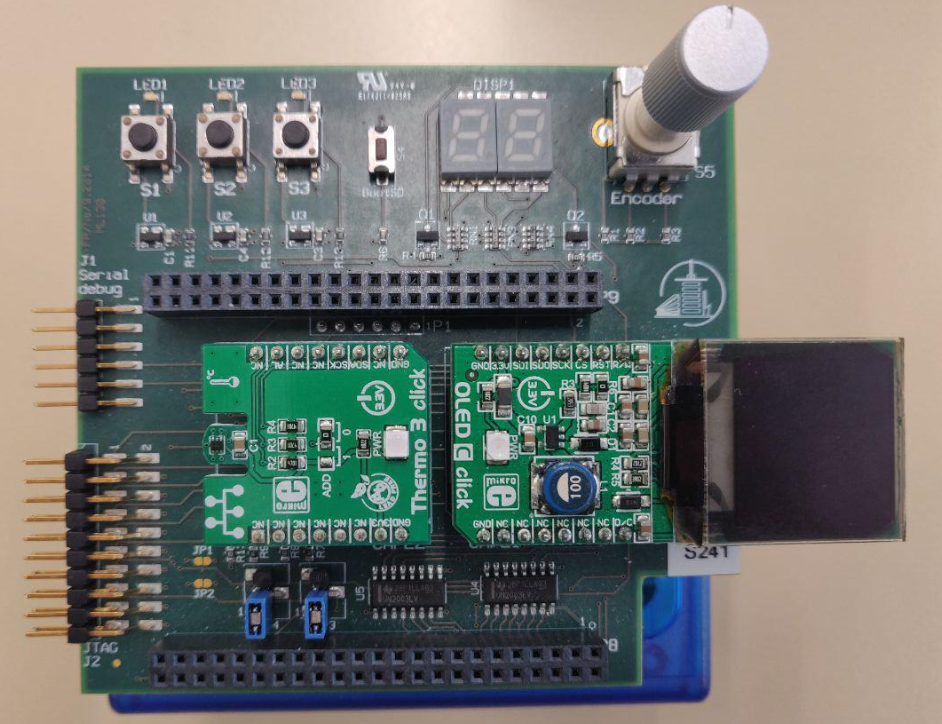
\includegraphics[scale=.5]{bbb.PNG}\\[1.5cm]
            \vspace*{1\baselineskip}
            \today \\[0.7cm]
        \end{center}
    \end{titlepage}
    \tableofcontents
    \clearpage
% \insertImage{Img/1.PNG}{echelle pour l'image (source = 1)}{texte dessous l'image}{référence vers l'objet}
\section{Heure de travail}
2 heures

\section{Introduction}
Ce projet intégré vous nous permettre de mettre en pratique des concepts étudiés durant les cours de systèmes embarqués 1 et 2 grâce à l'implémentation d'un système d'exploitation élémentaire (coopératif) et de mettre en oeuvre divers périphériques d'entrée/sortie et de communication.\\
Une liste des contraintes est donnée:
\begin{itemize}
   \item Mettre en oeuvre le système d'exploitation élémentaire coopératif
   \item Mettre en oeuvre le système de traitement des interruptions
   \item Structurer le logiciel en plusieurs tâches (threads)
   \item Mettre en oeuvre un système de communication entre les tâches (p.ex. message queue)
   \item Traiter les périphériques d'entrée/sortie en mode interruptif (GPIO)
\end{itemize}

Cette première partie du projet intégré va permettre de lister une série d'idées, d'en choisir une et de la spécifier. Le système peut intéragir avec tous les éléments de la beaglebone et doit au moins possédé le composant RFid click ou nRF T click

Nous avons choisit le composant RFid click et voici les différentes applications que nous avons trouvées pour notre RFID sont:

\begin{itemize}
    \item Système de connexion via RFID
    \item Simulation d'un système de domotique d'une maison
    \item Jeu de réflexe avec badges de différentes couleurs
    \item Porte monnaie électronique / système de paiement sans cash
\end{itemize}

Le choix sur lequel nous avons décidé de continuer est le \textbf{système de simulation de domotique d'une maison}.

\section{Synthèse}

\paragraph{Sven}

\textbf{\textit{Acquis}}
\begin{itemize}
    \item Trouver des idées
    \item Découpage en fonctions
\end{itemize}

\paragraph{Marc}

\textbf{\textit{Acquis}}
\begin{itemize}
    \item Mise en commun d'idées
    \item Reflexion autour d'un projet ou le sujet est libre
    \item Déterminer les fonctions nécessaires à notre implémentation
\end{itemize}


\newpage

\section{Périphériques utilisés}
Les différents périphériques que nous utiliser pour notre projet intégré sont:
\begin{itemize}
    \item Bouton S1
    \item Display DISP1
    \item Encodeur Encoder
    \item Leds LED1 LED2 LED3
    \item Display OLED 
    \item Tag RFID
    \item Module RFID
\end{itemize}
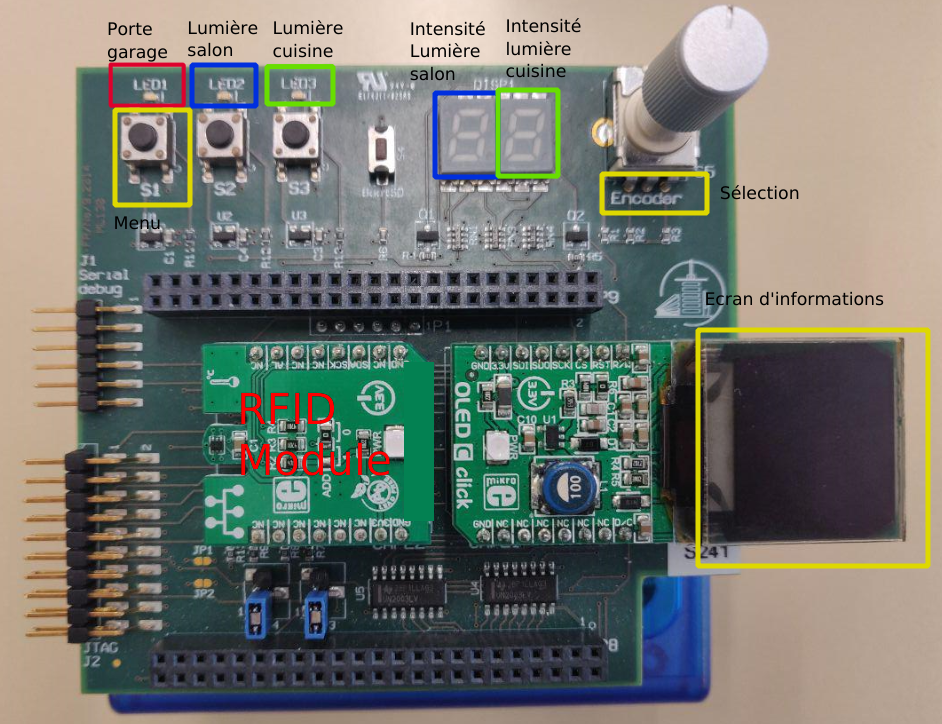
\includegraphics[width=1\textwidth]{bbbMod.png}

\section{Spécifications de notre projet}

Dans ce projet intégré nous allons réaliser une simulation de la domotique pour une maison. Le principe sera de se servir des différents badges RFID que l'utilisateur pourra lier à une fonction:
\begin{itemize}
    \item Intensité lumineuse cuisine, salon
    \item Réglage thermostat de la maison
    \item Possibilité de configurer de nouveaux badges librement
    \item Système de gestion des badges
    \item Ouverture/ fermeture de la porte du garage
\end{itemize}

\section{Fonctions à concevoir}
A l'initialisation le système affiche sur l'écran OLED un message de bienvenue affichant: \textbf{Présentez un badge} et il restera dans cet état tant que aucune badge ou le bouton S1 n'aura pas été préssé. C'est l'état de base

\subsection{Détection de badge}
Si un badge a été posé et détecté, il faut attendre que le système se retrouve dans son état de base pour pouvoir relancer la détection d'un badge, pour éviter des problèmes la détection des badges se fera uniquement dans l'état de base\\
Dans le cas ou un badge inconnu est apposé, un message demande: \textbf{Voulez vous ajouter ce badge ?} On peut ensuite choisir avec l'encodeur oui ou non et dans le cas où oui est sélectionné, on se retrouve dans le menu de configuration.

\subsection{Affichage séquence}
Lorsqu'un badge est détecté, l'action ou les actions définies sur ce badge sont effectuées et affichées sur l'écran OLED pendant un certain et après il retourne dans l'état de base affichant le message


\subsection{Les différents types de badges}
\begin{itemize}
    \item \textbf{Les Tags monofonction :} Associe à ce badge une seule action, par exemple la porte du garage
    \item \textbf{Les Tags multifonctions :} Associe le badge à une série d'action, par exemple la lumière du salon à 50\%, de la cuisine et ouverture de la porte du garage (si porte fermée). Le nombre d'action maximum est de 3 et toutes les actions peuvent être liées sauf le thermostat
\end{itemize}

\subsection{Porte du garage}
La LED1 de notre BeagleBone simulera la porte du garage, 1 si la porte est ouverte, 0 si fermée. \\\\
Pendant que la porte est en mouvement la LED1 clignote. On affichera aussi entre autre sur l'écran: \textbf{Ouverture/fermeture porte}.

\subsection{Fonction de réglage de l'intensité de la lumière}
La LED2 et la LED3 de notre BeagleBone simuleront respectivement la lumière du salon et la lumière de la cuisine et nous pourrons via l'encodeur régler l'intensité lumineuse.\\
Lorsque l'on rêgle l'intensité lumineuse du salon ou de la cuisine,l'affichage sur les digits du display s'affiche un certain temps avant de s'éteindre et que le système retourne dans son état de base.\\
On indiquera le niveau de l'intensité lumineuse sur le DISP1, chaque segment indique une intensité de 16\%. Lorsque l'intensité lumineuse sera maximale le digit correspondant formera un cercle complet. 


\subsection{Réglage du thermostat}
Lorsque l'on choisit de régler le thermostat, un thermomètre apparaît sur l' OLED et nous pourrons via l'encodeur régler le thermostat et valider la température avec le bouton de l'encodeur\\
L'affichage mis à jour en temps réel et lorsque la température voulue est atteinte, le thermomètre reste affiché un certain avant que le système retourne dans l'état de base

\subsection{Mode configuration des Badges}
Ce mode permet de gérer les badges\\
On rentre dans le mode configuration via la touche S1\\
Ensuite le menu s'affiche sur le LCD où il est possible de naviguer via l'encodeur et valider grâce à son bouton pour effectuer les différentes configurations:\\

Pour Ajouter un badge, sélectionner \textbf{Ajouter un badge}, présenter le badge et attendre le message de confirmation. Au moment d'ajouter le badge, on devra choisir dans le menu s'il sera mono ou multifonction, pour passer de mono à multi ou vice versa, il est nécessaire de supprimer le badge.\\
Il faut ensuite dans le menu sélectionner la ou les actions qui seront définies. \\
Dans le cas d'un badge monofonction, dès que l'action à été sélectionnée, l'écran affiche une confirmation et retourne dans son état de base. 
Si le badge est multifonction, il faut définir le nombre d'actions que l'on va lui lier et ensuite dès que une action a été liée, le système redemande de sélectionner l'action (comme pour un bagde monofonction) et ainsi de suite, jusqu'au moment où l'on va atteindre le nombre d'actions requises. Et il ensuite retourne dans l'état de bas\\
Pour supprimer le bagde du système, il faut sélectionner la fonction \textbf{Supprimer le badge} et présenter le badge.\\
Pour sortir du mode configuration, sélectionner la fonction \textbf{Quitter} du menu.
Durant la phase de liaison entre les actions et le badge, la détection d'autres badges est désactivée


\subsection{Fonctions supplémentaires}
\begin{itemize}
   \item Thermostat compris dans un badge multifonction
   \item Gestion à distance depuis un autre beaglebone
   \item Parallélistion des fonctions et détection multiples de badges
\end{itemize}

\section{Conclusion}
Cette partie nous a permis de bien spécifier ce que fera et ne fera pas notre application et va permettre au professeur de nous orienter dans le cas d'une application trop simple ou trop compliquée

\section{Pêchés capitaux}
\begin{itemize}
   \item L'Orgueil - livrer un programme sans vérification
   \item l'Avarice - écrire un code monolithique
   \item L'Envie - utiliser des nombres magiques
   \item La Colère - laisser les warnings à la compilation
   \item L'Inconsistance - mal indenter, choisir des noms inappropriés, etc.
   \item La Paresse - écrire un code sans commentaire
   \item La Gourmandise - copier du code sans citation
\end{itemize}

\end{document}
